%% REPLACE sXXXXXXX with your student number
\def\studentNumber{s1720422}


%% START of YOUR ANSWERS
%% Add answers to the questions below, by replacing the text inside the brackets {} for \youranswer{ "Text to be replaced with your answer." }. 
%
% Do not delete the commands for adding figures and tables. Instead fill in the missing values with your experiment results, and replace the images with your own respective figures.
%
% You can generally delete the placeholder text, such as for example the text "Question Figure 2 - Replace the images ..." 
%
% There are 19 TEXT QUESTIONS (a few of the short first ones have their answers added to both the Introduction and the Abstract). Replace the text inside the brackets of the command \youranswer with your answer to the question.
%
% There are also 3 "questions" to replace some placeholder FIGURES with your own, and 3 "questions" asking you to fill in the missing entries in the TABLES provided. 
%
% NOTE! that questions are ordered by the order of appearance of their answers in the text, and not by the order you should tackle them. Specifically, you cannot answer Questions 2, 3, and 4 before concluding all of the relevant experiments and analysis. Similarly, you should fill in the TABLES and FIGURES before discussing the results presented there. 
%
% NOTE! If for some reason you do not manage to produce results for some FIGURES and TABLES, then you can get partial marks by discussing your expectations of the results in the relevant TEXT QUESTIONS (for example Question 8 makes use of Table 1 and Figure 2).
%
% Please refer to the coursework specification for more details.


%% - - - - - - - - - - - - TEXT QUESTIONS - - - - - - - - - - - - 

%% Question 1:
\newcommand{\questionOne} {
\youranswer{when a network function is too closely fit to a training
set, and results in an increasing validaiton set error despite a
monotonically decreasing training error(an illustration
 of this concept is shown in figure 1b).}
}

%% Question 2:
\newcommand{\questionTwo} {
\youranswer{Question 2 - Summarise the effect increasing width and depth of the architecture had on overfitting}
}

%% Question 3:
\newcommand{\questionThree} {
\youranswer{Question 3 - Summarise what your results show you about the effect of the tested approaches on overfitting and the performance of the trained model}
}

%% Question 4:
\newcommand{\questionFour} {
\youranswer{Question 4 - Give your overall conclusions}
}

%% Question 5:
\newcommand{\questionFive} {
\youranswer{it's validation error begins to increase despite it's training
error decreasing monotonically. This leads to an increasing generealization
gap as the model is trained over a number of epochs. It inidcates that
the model is too flexible and doesn't fit to unseen data very well.}
}

%% Question 6:
\newcommand{\questionSix} {
\youranswer{Overfitting occurs due to a high variance being present within
the trained model. This is due to the model becoming overly complex and
fitting its degrees of freedom in such a way which closely resembles data
points present in the training data. The parameters of the model learn 
the detail and noise in the training data which results in a negative
performance when it comes to the gnerealization of the model and its 
ability to closely predict outputs on unseen data. Overfitting can occur
for a number of reasons. If the learing rate of a model is increased too
much, then it is likely that the parameters of the model will convege and resemble
training data points very closely in a fewer number of epochs respectively. A
clear way to identify if a model is overfit is by visualising the error of
the model on a training and vaildation set across a fixed number of epochs. If 
the validation error begins to increase despite a monotonically decreasing
training error, the model is said to be overfitted. To generalize, if the Model
performs well on a training set, but poorly on unssen data, it is overfitted. 
  }
}

%% Question 7:
\newcommand{\questionSeven} {
\youranswer{it highlights the ratio of total EMNIST samples which were
classified with their target labels correctly over a period of 100 epochs. the
red and blue lines rpresent the accuracy obtained by the baseline model across
the training and test set respectively. It cna be observed that the accuracy
of predictions steeply increased up until epoch 5. Beyond which training accuracy
continued to increase steeply in contrast to the validation accuracy which 
increased at a slower rate and began to level off. At around epoch 16, it
is clear that the model was no longer improving in validation accuracy due to a flat
gradient in the validation accuracy curve. This indicates a maximum optimum
accuracy of 82.5\% was achieved for the model at epoch 16 before it's performance
began to decline. Figure 1b similarly illustrates epoch 16 as the point where
the cross-entropy error measured on the validation set was at it's minimum of
0.5, before it begian to increase. It can be deduced that beyond epoch 16,
training accuracy continued to increase monotonically, whereas validation
accuracy began to decline. A similar pattern can be observed for figure 1b
where the error on the training set conintured to decrease beyond epoch 16,
whereas it increased for the validatoin set. This led to an expanidng
generalization gap. Hence, the baseline model became overfitted
beyond epoch 16. By the end of epoch 100, it can be seeen that the accuracy
across the validation set had fallen from 82.5\% to 80.5\%. Furthermore,
the error across the validation set increased from a minimum of 0.5 to
approximately 0.98. In contrast, by epoch 100, the training set was clearly
fitted to the model due to the high training accuracy of 93.5\% and low
error of 0.17.
}
}

%% Question 8:
\newcommand{\questionEight} {
\youranswer{as the number of hidden units is increased, this does lead to an
imprvement in validation accuracy, as shown in table 1.
The final validation accuracy increased from 78.5\% for 32
units to 80.3\$ for 128 units. We observe that the highest final
validation accuracy of 80.9\% was achieved using 64 hideen units. The reason
why the 128  uint model was unable to outperform the 64 units model is due To
overfititing.
Figure 2a and 2b shows that overfitting of the 128 model is indicated
by the rise in validation error(green line) beytond epoch 18, despite its's corresponding
training error decreasing(yellow line). This led to the decrease in validation accuracy
as shown in figure 2a for acccuraccies recorded beyond epoch 18.
By the end of epoch 100, we can see that the 64 units mode perfromed
almost identically to the 128 ubits model on the validation set.
 The 128 units model had
an advantage when it comes to how quickly the model converged and obtained lower
validation error and higher validation accuracies. It acheived
a maximum validation accuracy of approximately 82.5\% after epoch 18.
It was also the fastest model to see a drastic improvment in validation accuracy.
However due to overfitting, this afvantage didn't last too long. The 32 layer model 
perfomred the worst on the validation set and obtained the lwoest accuracy across the board. This 
is due to the model being underfit and not flexible enough to learn the parameters
needed to fit the training data well. Despite this, it did obtain the lowest
generalixation error of 0.15 so is the least likely model to result in
overfiting. In contrast, the 128 unit model is the most likely to overfit
due to a high geneeralization gap of 0.83.}
}

%% Question 9:
\newcommand{\questionNine} {
\youranswer{Varying the width affects the results in a consistent way as
expected. We expect the model to start off underfitted to the training data 
when less units are used. This is because the model is less
flexible due to having less free parameaters which can fit to to the data.
This is represented well with the lowest validation accutacy 
obtained in table 1 for the 32 units model.
As we increase the number of units. we expect the model to fit the inpuit data
better due to the model having increased flexibiliy. This is demonstrated 
successfully due to the 64 units model having obtained the best final vaildation
accuracy of all the models. Furthermore, we hypthesised that increasing the Model
flexibility too much and having a number of free paramters close to the number
of samples being trained on would result in overfitting due to each free parameters
closely fitting each training point, hence creating noise. This is clerarly 
demonstrated with the 128 units model in figure 2a where it's validation Accuracy
began to decrease despiute the trianing accuracy increasing. It is also clear
the model is overfit due to the increasing error generalization gap which had
formed. 
 }
}

%% Question 10:
\newcommand{\questionTen} {
\youranswer{across all 3 depths tested, the final validation accuracy of
each model increased as the model depth increased. This is primarily due to the
model converging quicker within a fixed amount of epochs as there are
more parameters being fitted to the training data. The consequence of 
increaisng depth is an increased generalizxation error gap. This can be seen from
the spread between the orange and green lines in figure 3a for the model of depth3
3. It mneans although the final validation accuracy increases, as depth increases,
the amount the model is overift by increases too hence causes the model to generalize
worse on unseen data. From figure 3b, we can see that the model of depth 1 has
the smallest generalization gap, whereas the model of depth 3 has the largest.
Furthermore, we can observe the effect of increasing depth to be marignal when
it comes to validation accuracy. This can be explained by the model of depth 1 hving
d a similar final
validation accurtacy of 81.2\% compared to the model of depth 2 and 3 which 
had accuraccies of 81.5\% and 82.0\% respectively. Therefore from figure 3a and
3b, we can conclude that increasing model complexity by increasing the depth
is counter-intuitive to imporving the generalization and validation accuracy of
the model. The model genrealizes better with a depth of 1, comparted to depth of
2 and 3. The validation acuttacy gain of using greater depths is marginal and
makes for a worse generalized model.
}
}

%% Question 11:
\newcommand{\questionEleven} {
\youranswer{Question 11 - Discuss whether varying depth affects the results in a consistent way, and whether the results are expected and match well with the prior knowledge (by which we mean your expectations as are formed from the relevant Theory and literature)}
}

%% Question 12:
\newcommand{\questionTwelve} {
\youranswer{Question 12 - Compare and discuss how varying width and height changes the performance and overfitting in your experiments}
}

%% Question 13:
\newcommand{\questionThirteen} {
\youranswer{Question 13 - Explain L1/L2 weight penalties first in words and then with formulas. Explain how they are incorporated to training and what hyperparameter(s) they require}
}

%% Question 14:
\newcommand{\questionFourteen} {
\youranswer{Question 14 - Discuss how/why the weight penalties may address overfitting, discuss how L1 and L2 regularization differ and support your claims with references where possible}
}

%% Question 15:
\newcommand{\questionFifteen} {
\youranswer{Question 15 - Explain the experimental details (e.g. hyperparameters), discuss the results in terms of their generalization performance and overfitting}
}

%% Question 16:
\newcommand{\questionSixteen} {
\youranswer{Question 16 - Explain the motivation behind Maxout Networks as presented in \cite{goodfellow2013maxout}}
}

%% Question 17:
\newcommand{\questionSeventeen} {
\youranswer{Question 17 - State whether Dropout is compatible (can be used together) with Maxout and explain why}
}

%% Question 18:
\newcommand{\questionEighteen} {
\youranswer{Question 18 - Give an overview of the experiment setup in \cite{goodfellow2013maxout} and analyse it from the point of view of how convincing their conclusions are}
}

%% Question 19:
\newcommand{\questionNineteen} {
\youranswer{Question 19 - Briefly draw your conclusions based on the results from the previous sections (what are the take-away messages?) and conclude your report with a recommendation for future directions}
}


%% - - - - - - - - - - - - FIGURES - - - - - - - - - - - - 

%% Question Figure 2:
\newcommand{\questionFigureTwo} {
\youranswer{Question Figure 2 - Replace the images in Figure 2 with figures depicting the accuracy and error, training and validation curves for your experiments varying the number of hidden units.
%
\begin{figure}[t]
    \centering
    \begin{subfigure}{\linewidth}
        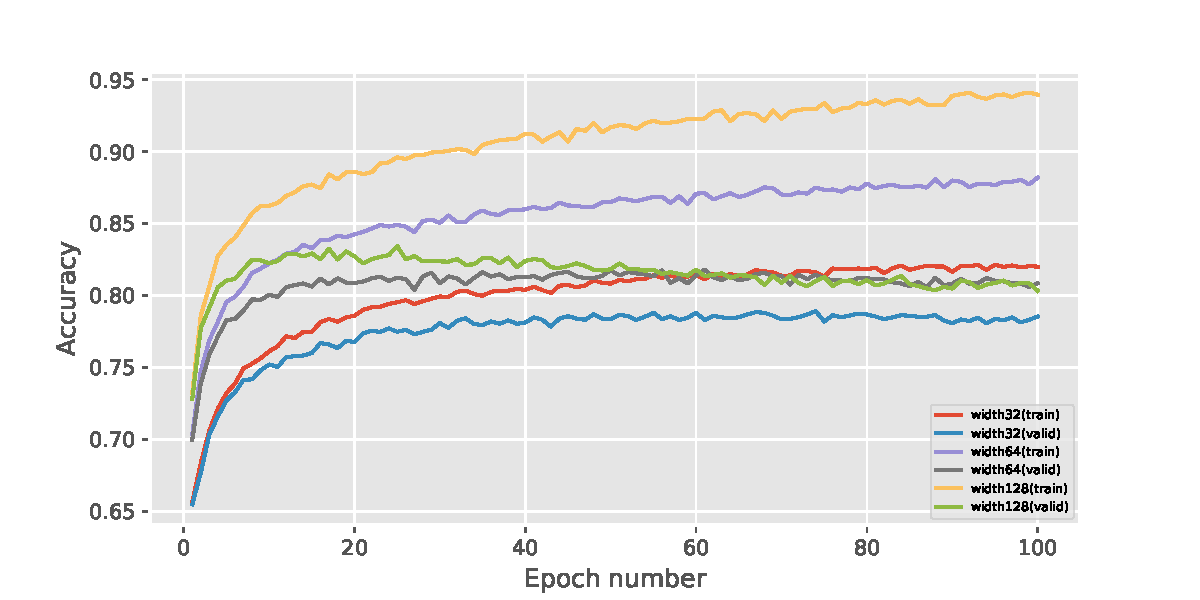
\includegraphics[width=\linewidth]{figures/task1_hu_accuracy.pdf}
        \caption{accuracy by epoch}
        \label{fig:width_acccurves}
    \end{subfigure} 
    \begin{subfigure}{\linewidth}
        \centering
        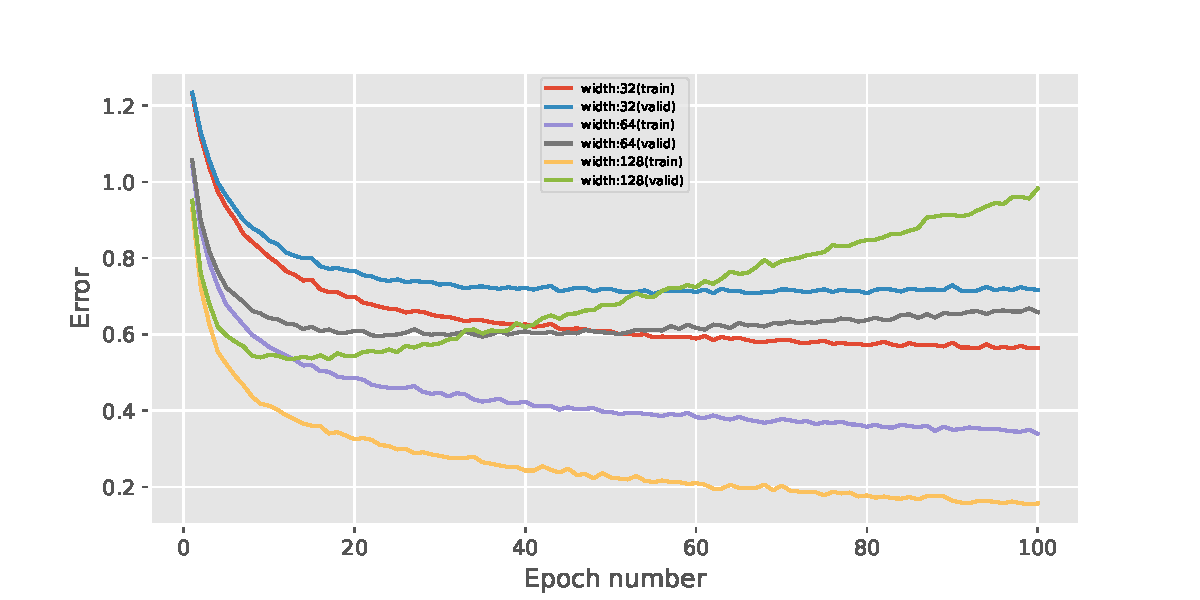
\includegraphics[width=\linewidth]{figures/task1_hu_error.pdf}
        \caption{error by epoch}
        \label{fig:width_errorcurves}
    \end{subfigure} 
    \caption{Training and validation curves in terms of classification accuracy (a) and cross-entropy error (b) on the EMNIST dataset for different network widths.}
    \label{fig:width}
\end{figure} 
}
}

%% Question Figure 3:
\newcommand{\questionFigureThree} {
\youranswer{Question Figure 3 - Replace these images with figures depicting the accuracy and error, training and validation curves for your experiments varying the number of hidden layers.
%
\begin{figure}[t]
    \centering
    \begin{subfigure}{\linewidth}
        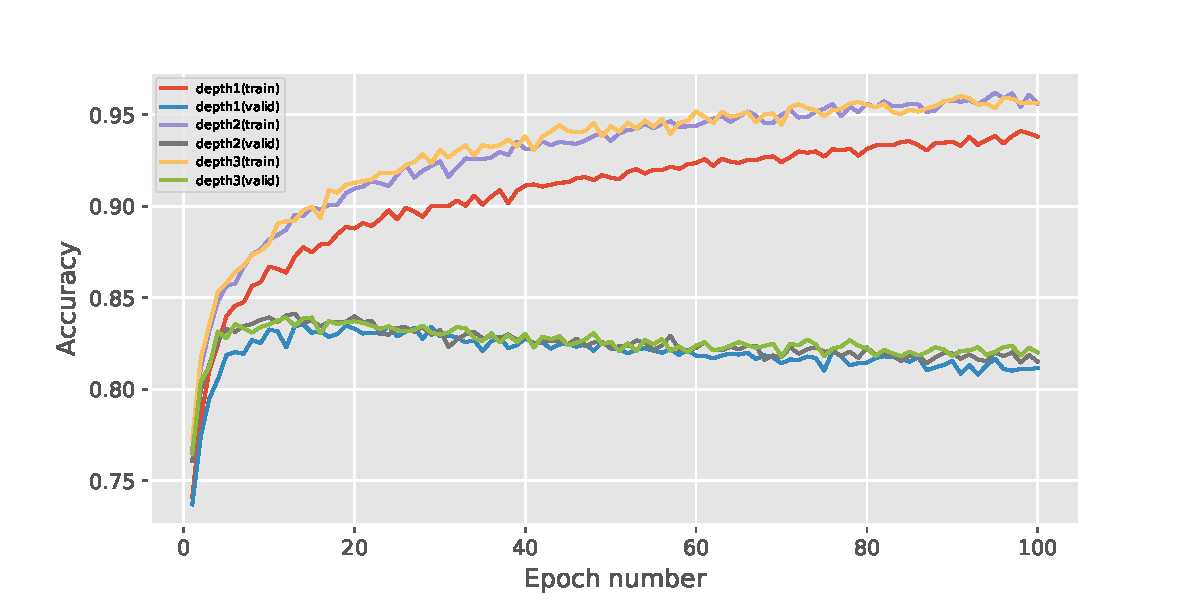
\includegraphics[width=\linewidth]{figures/task1_vlayers_accuracy.pdf}
        \caption{accuracy by epoch}
        \label{fig:depth_acccurves}
    \end{subfigure} 
    \begin{subfigure}{\linewidth}
        \centering
        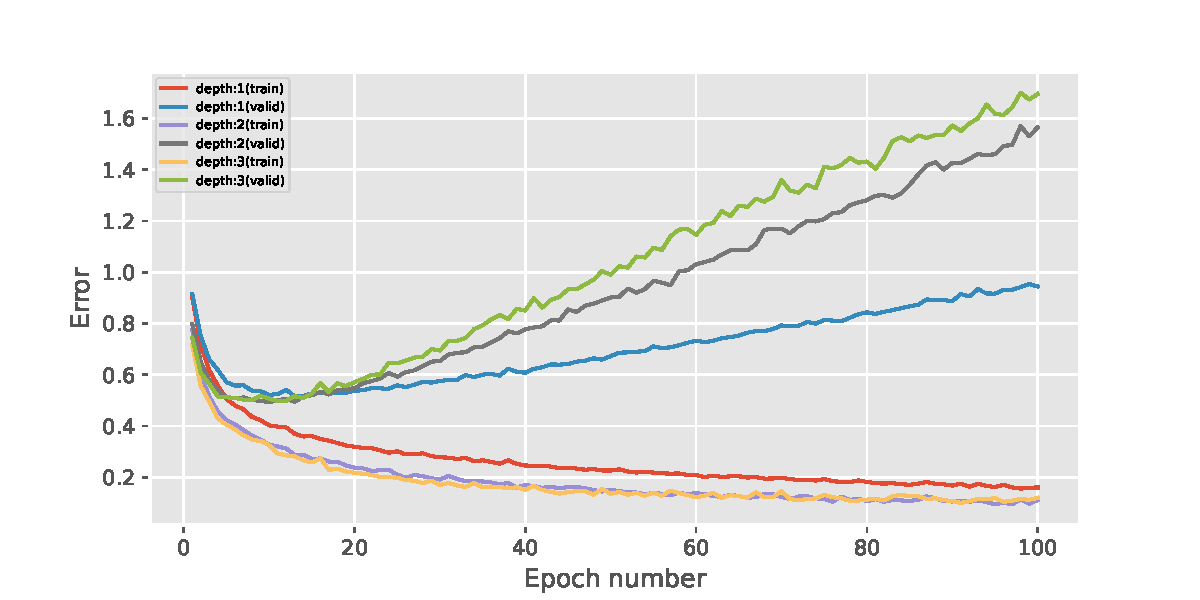
\includegraphics[width=\linewidth]{figures/task1_vlayers_error.pdf}
        \caption{error by epoch}
        \label{fig:depth_errorcurves}
    \end{subfigure} 
    \caption{Training and validation curves in terms of classification accuracy (a) and cross-entropy error (b) on the EMNIST dataset for different network depths.}
    \label{fig:depth}
\end{figure} 
}
}

%% Question Figure 4:
\newcommand{\questionFigureFour} {
\youranswer{Question Figure 4 - Replace these images with figures depicting the Validation Accuracy and Generalisation Gap for each of your experiments varying the Dropout inclusion rate, L1/L2 weight penalty, and for the 8 combined experiments (you will have to find a way to best display this information in one subfigure).
%
\begin{figure*}[t]
    \centering
    \begin{subfigure}{.3\linewidth}
        \includegraphics[width=\linewidth]{figures/empty_dropout_plot.png}
        \caption{Metrics by inclusion rate}
        \label{fig:dropoutrates}
    \end{subfigure} 
    \begin{subfigure}{.3\linewidth}
        \centering
        \includegraphics[width=\linewidth]{figures/empty_wd_plot.png}
        \caption{Metrics by weight penalty}
        \label{fig:weightrates}
    \end{subfigure} 
    \begin{subfigure}{.3\linewidth}
        \centering
        \includegraphics[width=.85\linewidth]{example-image-duck}
        \caption{Extra experiments}
        \label{fig:extra}
    \end{subfigure} 
    \caption{Hyperparameter search for every method and combinations}
    \label{fig:hp_search}
\end{figure*}
}
}

%% - - - - - - - - - - - - TABLES - - - - - - - - - - - - 

%% Question Table 1:
\newcommand{\questionTableOne} {
\youranswer{
Question Table 1 - Fill in Table 1 with the results from your experiments varying the number of hidden units.
%
\begin{table}[t]
    \centering
    \begin{tabular}{c|cc}
    \toprule
        \# hidden units & val. acc. & generalization gap \\
    \midrule
         32            &        78.5    &            0.15        \\
         64            &        80.9   &             0.32       \\
         128           &        80.3  &              0.83      \\ 
    \bottomrule
    \end{tabular}
    \caption{Validation accuracy (\%) and generalization gap (in terms of cross-entropy error) for varying network widths on the EMNIST dataset.}
    \label{tab:width_exp}
\end{table}
}
}

%% Question Table 2:
\newcommand{\questionTableTwo} {
\youranswer{
Question Table 2 - Fill in Table 2 with the results from your experiments varying the number of hidden layers.
%
\begin{table}[t]
    \centering
    \begin{tabular}{c|cc}
    \toprule
        \# hidden layers & val. acc. & generalization gap \\
    \midrule
         1               &      81.2      &       0.78             \\
         2               &      81.5      &        1.46            \\
         3               &      82.0     &         1.58           \\ 
    \bottomrule
    \end{tabular}
    \caption{Validation accuracy (\%) and generalization gap (in terms of cross-entropy error) for varying network depths on the EMNIST dataset.}
    \label{tab:depth_exps}
\end{table}
}
}

%% Question Table 3:
\newcommand{\questionTableThree} {
\youranswer{
Question Table 3 - Fill in Table 3 with the results from your experiments varying the hyperparameter values for each of L1 regularisation, L2 regularisation, and Dropout (use the values shown on the table) as well as the results for your experiments combining L1/L2 and Dropout (you will have to pick what combinations of hyperparameter values to test for the combined experiments; each of the combined experiments will need to use Dropout and either L1 or L2 regularisation; run an experiment for each of 8 different combinations). Use \textit{italics} to print the best result per criterion for each set of experiments, and \textbf{bold} for the overall best result per criterion.
%
\begin{table*}[t]
    \centering
    \begin{tabular}{c|c|cc}
    \toprule
        Model    &  Hyperparameter value(s) & Validation accuracy & Generalization gap \\
    \midrule
    \midrule
        Baseline &  -                    &               0.836 &                 0.290 \\
    \midrule
        \multirow{3}*{Dropout}
                 & 0.7                   &                     &                   \\
                 & 0.9                   &                     &                   \\
                 & 0.95                  &                     &                   \\
    \midrule
        \multirow{3}*{L1 penalty}
                 & 1e-4                   &                     &                   \\
                 & 1e-3                   &                     &                   \\
                 & 1e-1                   &                     &                   \\
    \midrule
        \multirow{3}*{L2 penalty}  
                 & 1e-4                   &                     &                   \\
                 & 1e-3                   &                     &                   \\
                 & 1e-1                   &                     &                   \\
    \midrule
        \multirow{6}*{Combined}  
                 & for example 0.95, L1 1e-6  &                     &                   \\
                 & ?, ?                   &                     &                   \\
                 & ?, ?                   &                     &                   \\
                 & ?, ?                   &                     &                   \\
                 & ?, ?                   &                     &                   \\
                 & ?, ?                   &                     &                   \\
    \bottomrule
    \end{tabular}
    \caption{Results of all hyperparameter search experiments. \emph{italics} indicate the best results per series and \textbf{bold} indicate the best overall}
    \label{tab:hp_search}
\end{table*}
}
}

%% END of YOUR ANSWERS